\chapter{サーバーゾーンでのクラスタ構築}
\label{chap:fourth}

\section{緒言}
本章ではサーバーゾーンでのクラスタ構築について述べる.

\section{Elasticsearchのバージョンアップ}
3章の検証結果より, 異なるバージョンのElasticsearchノードでクラスタを構築することは出来ないため, リサイクル館の太陽光パネルの計測データを保存しているElasticsearch(133.71.201.197)をバージョンアップする必要がある. そこで, 133.71.201.197にインストールされたElasticsearchのバージョンアップを行う.

\section{バージョンアップ手順}

\subsection{インストール方法の特定}

バージョンアップを行うためには, 133.71.201.197のUbuntuPCにどのようにElasticsearchをインストールしたか特定する必要がある.

図 \ref{4-p1}に, aptによってインストールされたパッケージの中にelasticsearchという文字列を含むパッケージが存在するか調べた結果を示す.
図 \ref{4-p1}より, aptによってインストールされたことが分かった.

\begin{figure}
  \begin{center}
    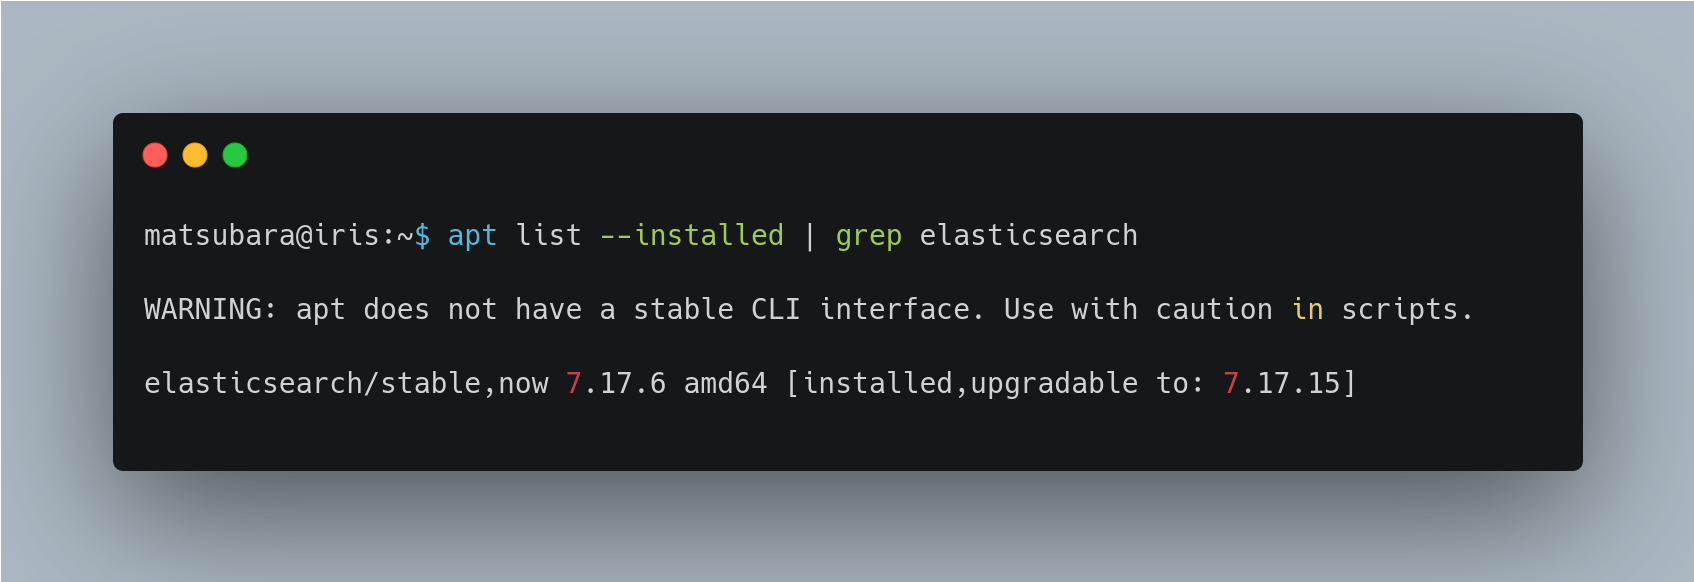
\includegraphics[width=160mm]{sotu/figure/apt-grep.png}
    \caption{aptによってelasticsearchがインストールされたか調べた結果}
    \label{4-p1}
  \end{center}
\end{figure}

次に, aptでインストール可能なelasticsearchのバージョンを一覧表示した結果を図 \ref{4-p2}に示す. 図 \ref{4-p2}にターゲットである7.17.9が含まれているため, aptを使用してバージョンアップできることが確認できた.

\begin{figure}
  \begin{center}
    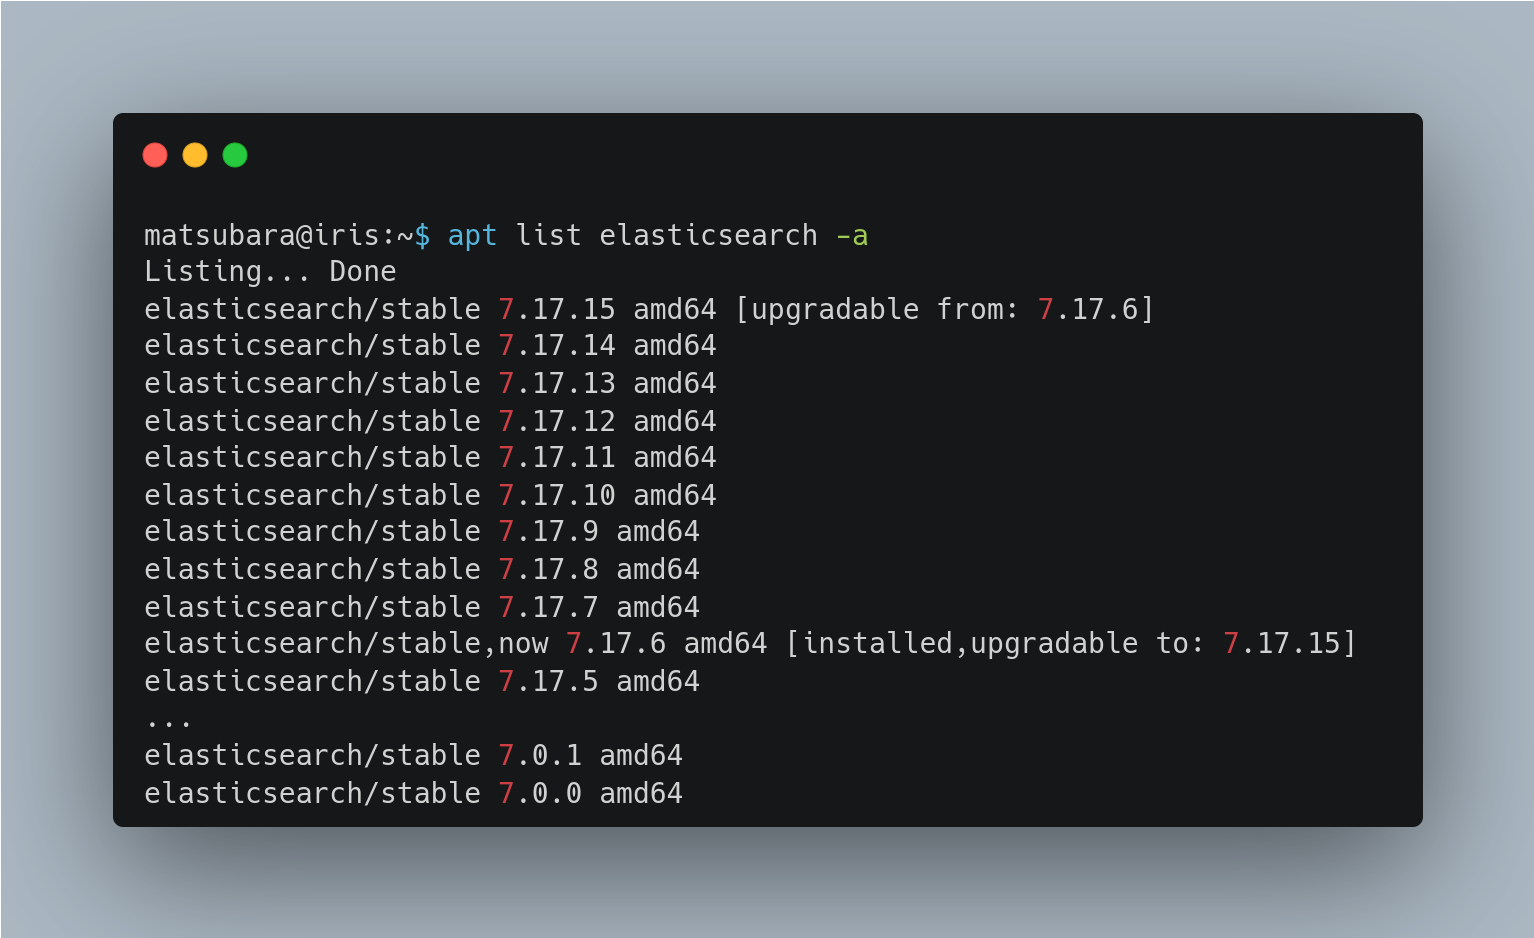
\includegraphics[width=160mm]{sotu/figure/apt-list.png}
    \caption{aptでインストール可能なelasticsearchのバージョンを一覧表示した結果}
    \label{4-p2}
  \end{center}
\end{figure}

\subsection{aptによるバージョンアップ}

まず, \textbf{sudo systemctl stop elasticsearch.service}コマンドを実行してelasticsearchノードをシャットダウンする.

次に, \textbf{sudo apt install elasticsearch=7.17.9}コマンドを実行してelasticsearchパッケージをバージョンアップする.

elasticsearchをバージョンアップ後, \textbf{sudo systemctl start elasticsearch}コマンドを実行してElasticsearchノードを起動する.

ノードの起動後, Elasticsearchのバージョンを確認した結果を図 \ref{4-p3}に示す.

\begin{figure}
  \begin{center}
    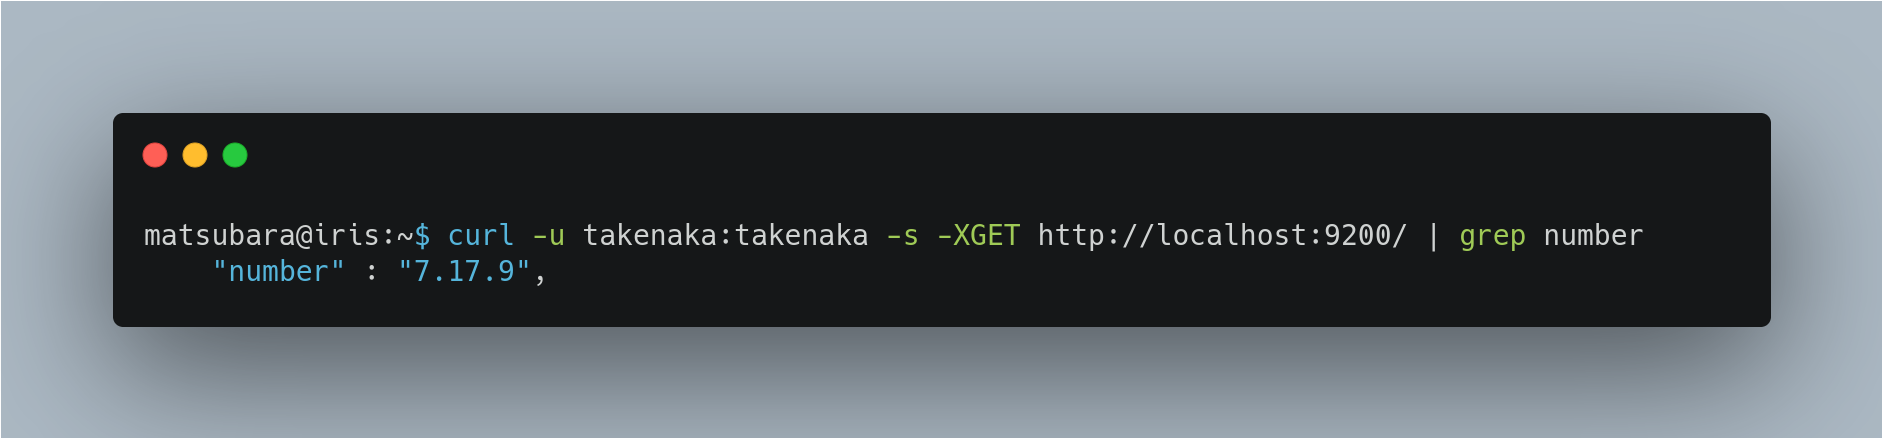
\includegraphics[width=160mm]{sotu/figure/version-check.png}
    \caption{ノードの起動後, Elasticsearchのバージョンを確認した結果}
    \label{4-p3}
  \end{center}
\end{figure}

図 \ref{4-p3}より, Elasticsearchのバージョンが7.17.9にバージョンアップ出来たことが確認できた.

\section{kibanaのバージョンアップ}

kibanaもelasticsearchと同様, aptを使用してインストールされていたため, \textbf{sudo systemctl stop kibana.service}コマンド, \textbf{sudo apt install kibana=7.17.9}コマンド, \textbf{sudo systemctl start kibana}コマンドをそれぞれ実行して, kibanaのバージョンアップも行った.

\section{バージョンアップ後の動作確認}

Elasticsearchのバージョンアップ後, 太陽光パネルの計測データがElasticsearchに保存されているかkibana上で確認した結果を図 \ref{p4}に示す.

\begin{figure}
  \begin{center}
    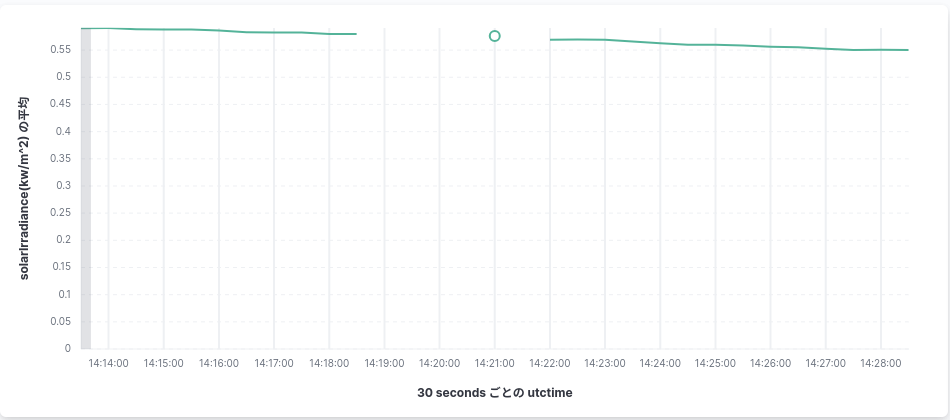
\includegraphics[width=160mm]{sotu/figure/downtime.png}
    \caption{Elasticsearchのバージョンアップ後, 太陽光パネルの計測データが保存されているかkibana上で確認した結果}
    \label{4-p4}
  \end{center}
\end{figure}

図 \ref{4-p4}より, バージョンアップ後のElasicsearchノードを起動した14:22:00以降にドキュメントがインサートされていることが確認できた.

\section{サーバーゾーンにおけるクラスタの構築}

\section{結言}
本章ではサーバーゾーンでのクラスタ構築について述べた.

次章では結論と今後の課題について述べる.